\documentclass{llncs}
% Grundgröße 12pt, zweiseitig
% Standardpakete
% richtiges encoding fuer verschiedene compiler
\usepackage{iftex}
\ifPDFTeX
   \usepackage[utf8]{inputenc}
   \usepackage[T1]{fontenc}
   \usepackage{lmodern}
\else
   \ifXeTeX
     \usepackage{fontspec}
   \else 
     \usepackage{luatextra}
   \fi
   \defaultfontfeatures{Ligatures=TeX}
\fi
% deutsche Silbentrennung
\usepackage[english]{babel}
\usepackage{amsmath}
\usepackage{cite}
\usepackage{float}
\usepackage{subfig}

% Grafiken einbinden
\usepackage{graphicx}
\graphicspath{{figures/}}

\usepackage{hyperref}
% tiefe des Inhaltsverzeichnisses
\setcounter{tocdepth}{2}


\begin{document}

\title{Comparative exploration of Abalone game-playing agents}
\author{Ture Claußen, 202132027, \email{ture.claussen@stud.hs-hannover.de}}
\authorrunning{T. Claußen}
\institute{Dept. of Software and Computer Engineering, Ajou University}

% jetzt gehts los
{\def\addcontentsline#1#2#3{}\maketitle} % Wird gebraucht, damit der Title nicht im Inhaltsverzeichnis steht

\begin{abstract}
  Games provide the perfect environment for artificial agents to navigate in. Especially for the
  \keywords{AI \and Alpha-beta \and Q-Learning \and Abalone \and Intelligent Agents}
\end{abstract}

\section{Introduction}

Abalone is a fairly new game, that was devised in 1987 by Michel Lalet and Laurent Lévi. Nevertheless, with more than four million global sales it could establish itself as a classic game \cite{noauthor_abalone_2020}. Ablalone is a two-player game consisting of a hexagonal board with 61 fields and 14 marbles for black and white respectively. The abstract nature of the game requires the player to plan ahead and find the right strategy in the plethora of moves. The goal is to create an agent that is up to par with a human player and moreover, has realistic computational requirements and reacts quickly.

In search of the optimal move it is not possible to expand all of the possible paths the game could take, even for modern computers. Hence, more sophisticated approaches for navigating the state space and evaluating good paths are needed. On the other hand, the game does not have piece-specific rules or large distance moves which reduces the need for a very domain specific knowledge about the game like e.g. for chess to find sensible heuristics.

\subsection{Motivation}
Overall, this degree of complexity makes the game a good project for the design of a game playing-agent, as it is meant to be an opportunity to apply the fundamental principles and algorithms learned in the class, as opposed to being distracted by the engineering aspects. This matches my personal background on the subject matter, as I have no prior (formal) exposure to the design of artificial intelligence. In addition, this project is only created for the purpose of this class. Over the course of my current study of applied computer science I gained versatile proficiency in programming and the handling of data which will help implementing the algorithms efficiently and provide the empirical foundation for the paper.

\subsection{Survey}

Considering the existing landscape of papers, there is unquestionably a wide array of papers exploring the application of minimax and alpha-beta pruning on the game of Abalone. Some of the most prominent include:

\begin{enumerate}
  \item "Algorithmic fun-abalone" (2002) Considers foundational heuristics for the game and analyzes minimax and its refinements in the form of (heuristic) alpha-beta pruning. Furthermore it sheds light on the performance differences between those. \cite{aichholzer_algorithmic_2002}
  \item "A Simple Intelligent Agent for Playing Abalone Game: ABLA" (2004) Implementation of a game-playing agent with minimax, alpha-beta pruning and some custom heuristics. The evaluation of the performance is done by comparing the agent to existing software in the form of ABA-PRO and RandomSoft.\cite{ozcan_simple_2004}
  \item "Constructing an abalone game-playing agent" (2005) Provides a very thorough explanation and analysis of the game's fundamentals, such as the state space, rules and positions. In regards to the alpha-beta pruning it also explains strategies for ordering the nodes and performance concerns. \cite{lemmens_constructing_2005}
  \item "Implementing a computer player for abalone using alpha-beta and monte-carlo search" (2009) This master thesis is a very exhaustive analysis of the game, alpha-beta pruning and Monte Carlo tree search, conferring many of the previous results. \cite{chorus_implementing_2009}
\end{enumerate}

These resources give great insight into the classical approaches, but they are lacking certain qualities:
\begin{itemize}
  \item Accessible and freely explorable code that underlies the analysis
  \item Comparision with modern approaches like Q-Learning that might reduce the resource demand on the client side
\end{itemize}

The proposed project seeks to build upon the given insight to improve upon these missing qualities.

\subsection{Rules}
The goal of the game is to push six of the opponent's marbles off the playing field. The game's starting position is depicted in figure \ref{basics} (a). One, two, or three adjacent marbles (of the player's own color) may be moved in any of the six possible directions during a player's turn. We differentiate between broadside or "side-step" moves and "in-line" moves, depending on how the chain of marbles moves relative to its direction, which is shown in figure \ref{basics} (b) and (c).

\begin{figure}[!h]
  \centering
  \subfloat[Starting position]{
    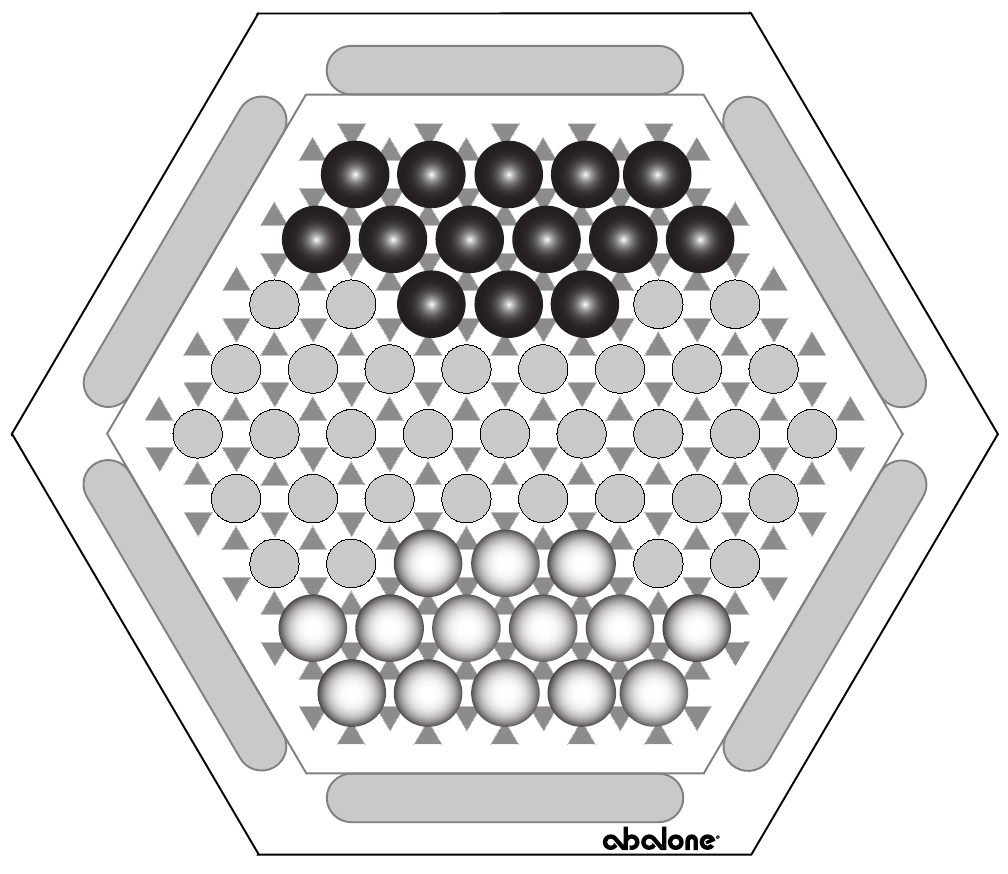
\includegraphics[width=3cm, keepaspectratio]{rules_starting_position.png}
  }
  \hfill
  \subfloat["In-line" moves]{
    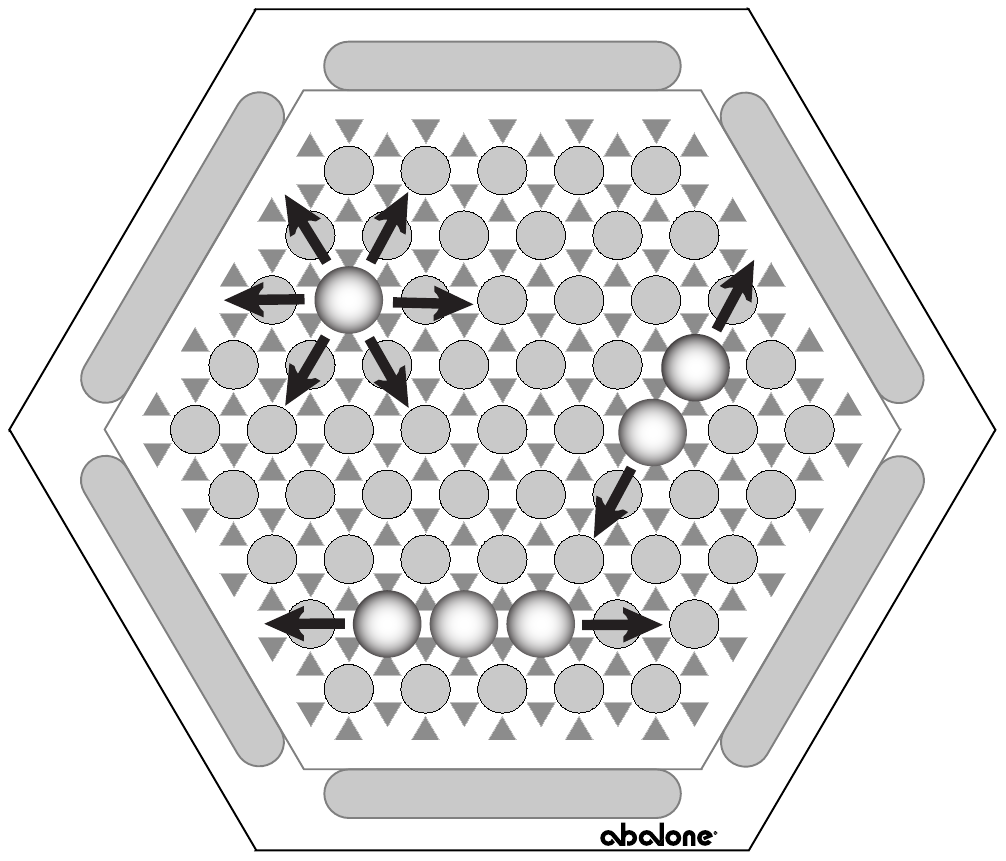
\includegraphics[width=3cm, keepaspectratio]{rules_inline_move.png}
  }
  \hfill
  \subfloat["Side-step" moves]{
    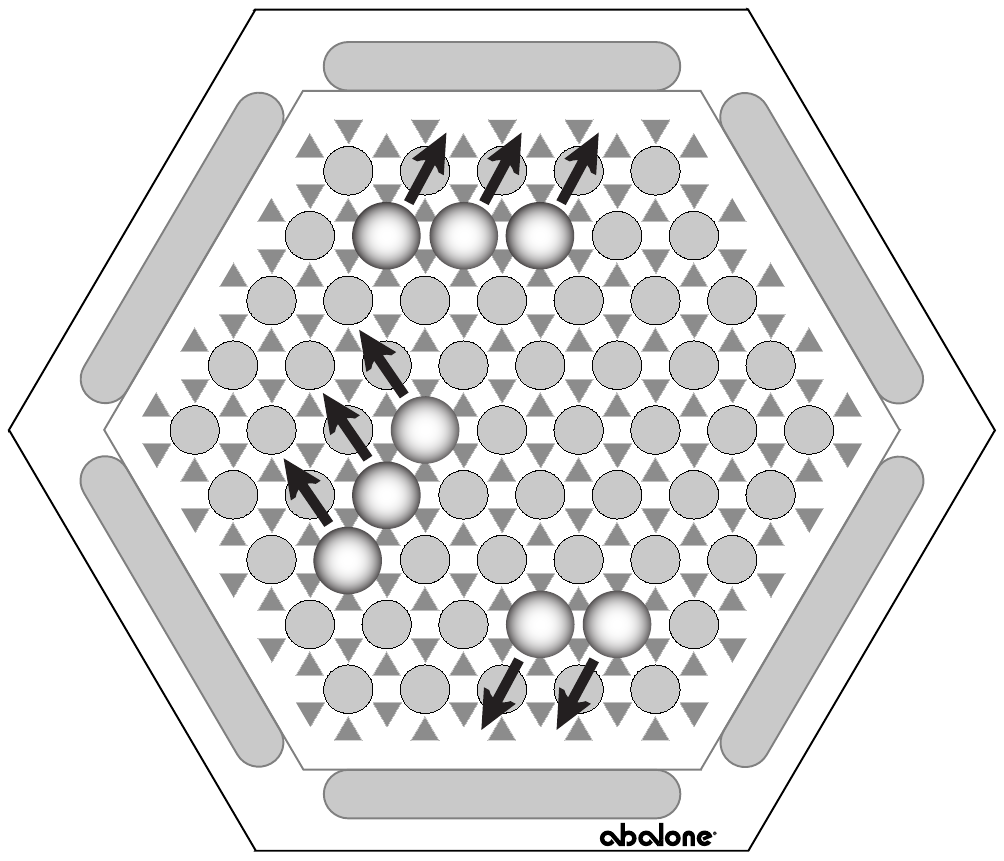
\includegraphics[width=3cm, keepaspectratio]{rules_side_step_move.png}
  }
  \caption{Basic moves \cite{abalone_sa_abalone_nodate}}
  \label{basics}
\end{figure}

A move pushing the opponent's marbles is called "sumito" and comes in three variations, as shown by figure \ref{sumito}. Essentially, the player has to push with superior numbers and the oponent's marbles can not be blocked. This is the game mechanic that allows for pushing the marbles out of the game and winning.

\begin{figure}[!h]
  \centering
  \subfloat["2-push-1" sumito]{
    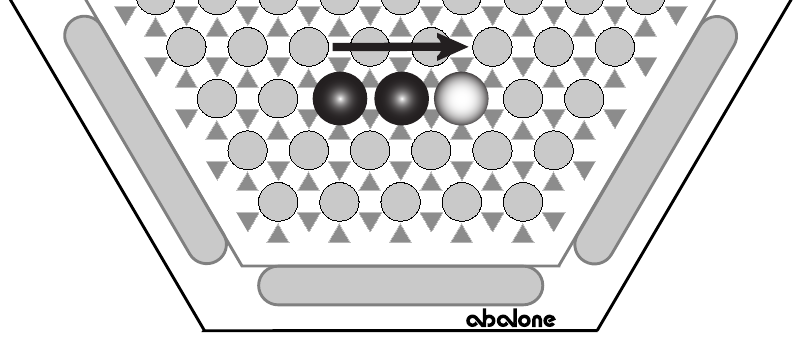
\includegraphics[width=3cm, keepaspectratio]{rules_2-push-1_sumito.png}
  }
  \hfill
  \subfloat["3-push-1" sumito]{
    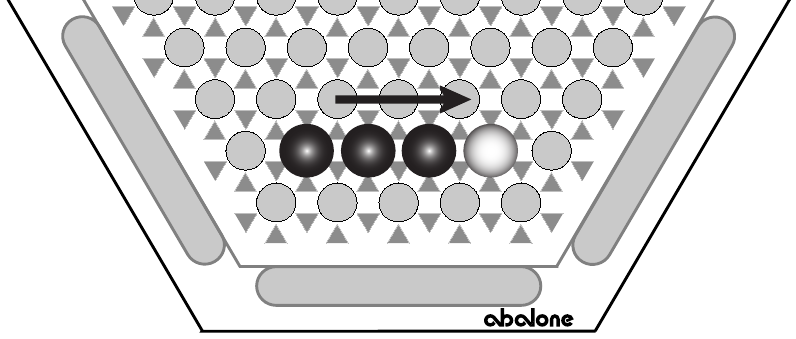
\includegraphics[width=3cm, keepaspectratio]{rules_3-push-1_sumito.png}
  }
  \hfill
  \subfloat["3-push-2" sumito]{
    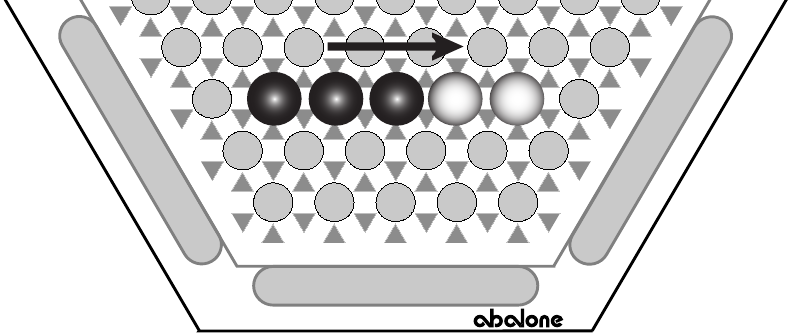
\includegraphics[width=3cm, keepaspectratio]{rules_3-push-2_sumito.png}
  }
  \caption{Sumito positions allow pushing the opponent's marbles \cite{abalone_sa_abalone_nodate}}
  \label{sumito}
\end{figure}

\section{Project details}

\subsection{Agent design}

Based on the PEAS framework we can analyze the task environment for the agent. \cite[p.107]{russell_artificial_2021}

\begin{description}
  \item[Performance measure] Win/loss, number of moves, time to deliberate
  \item[Environment] Digital playing board
  \item[Actuators] Move marbles, display text to CLI
  \item[Sensors] Position of marbles
\end{description}

\subsection{Complexity}
An important characteristic of a game environment is its complexity, which can be described two relevant dimensions.

\paragraph{State space complexity}

The state space is the collection of all possible state the agent can be in.\cite[p. 150]{russell_artificial_2021} For Abalone this means we have to consider all possible board configurations with different numbers of marbles present. Additionally, we would have to correct duplicates, that arise from the symmetries of the board. Ignoring this fact the following gives a good upper bound:

$$
  \sum_{k=8}^{14}\sum_{m=9}^{14}\frac{61!}{k!(61-k)!}\times\frac{(61-k)!}{m!((61-k)-m)!}
$$

\paragraph{Game tree complexity} The game tree defines the dependencies between board positions (nodes) and moves (edges). First we consider the branching factor (how many moves are possible in one position) of the game tree, which is on average 60.  \cite{lemmens_constructing_2005}

Putting Abalone's complexity in relation with other popular games, its state space complexity is on the same level as Reversi, whilst its game tree surpasses chess in complexity (c.f. table \ref{complexity_table})

\begin{table}
  \begin{center}
    \begin{tabular}{ | c | c | c | }
      \hline
      Game        & state-space complexity (log) & game-tree complexity (log) \\
      \hline
      Tic-tac-toe & 3                            & 5                          \\
      \hline
      Reversi     & 28                           & 58                         \\
      \hline
      Chess       & 46                           & 123                        \\
      \hline
      Abalone     & 24                           & 154                        \\
      \hline
      Go          & 172                          & 360                        \\
      \hline
    \end{tabular}
  \end{center}
  \caption{Abalone in comparision with other games \cite{chorus_implementing_2009}}
  \label{complexity_table}
\end{table}

\subsection{Algorithm comparision}
The main goal of the project is to compare several algorithmic approaches for the game-playing agent. The approaches shall be evaluated and compared in their:

\begin{itemize}
  \item Win/Loss-ratio
  \item Time to deliberate
\end{itemize}


\paragraph{Alpha-beta pruning}
This is the most explored and classical approach, wherefore it will form the baseline for the comparision. It will be necessary to find solutions on how to deal with the complexity of the game tree, such as iterative deepening, ordering of the nodes or various heuristics.

\paragraph{Monte Carlo Tree Search}
There are many strategies on how to implement the concept of Monte Carlo tree search, in this analysis the simplest approach will be utilized: Simulation of a certain amount of games to decide the next move.

\paragraph{Q-Learning}
Even though this class does not look at reinforcement methods in particular, Q-Learning seems to be a suitable method for a machine-learning based agent. The fact that it is a more simple algorithm, should allow for a timely implementation.

All three algorithms will be implemented from scratch, and played against each other. For the game environment several (python) libraries have been evaluated, namely "haliotis" \cite{noauthor_peer_nodate}, "Gym abalone" \cite{towzeur_towzeurgym-abalone_2021} and "Abalone BoAI" \cite{scriptim_scriptimabalone-boai_2021}. Both gym abalone and BoAI are specifically geared for the testing of intelligent agents, however, gym abalone is heavily focused on reinforcement-learning. Therefore, BoAI offers the simpler solution. If the gathering of empirical data or the training of the Q-Learning agent require computational resources, that exceed the ability of my personal Laptop, there is a budget of 30USD for buying compute time on a server.

\subsection{Timeline}

\begin{table}
  \begin{center}
    \begin{tabular}{ | c | c | c | }
      \hline
      Date  & Goal                                                  \\
      \hline
      05/03 & Design of heuristics, plan and setup code environment \\
      \hline
      05/10 & Implementation of alpha-beta pruning agent            \\
      \hline
      05/17 & Implementation of MCTS agent                          \\
      \hline
      05/24 & Acquisition of background knowledge for Q-Learning    \\
      \hline
      05/31 & Implementation of Q-Learning agent                    \\
      \hline
      06/07 & Agent face-off, collection of data                    \\
      \hline
      06/15 & Project report and record presentation                \\
      \hline
    \end{tabular}
  \end{center}
\end{table}

\subsection{Potential difficulties}
There is certain risks involved with the project. First and foremost it is the Q-Learning agent could pose problems, as I am still unfamiliar with the implementation. Moreover, the library BoAI is not very popular, so there might be unexpected behavior down the line.

\section{Conclusion}

% Literatur
\bibliographystyle{splncs04.bst}
\bibliography{ref.bib}
\end{document}